\chapter{CTMQC applied to the Tully Models}
\label{chap:tully_models}

The Tully models, first proposed by John Tully in 1990 \cite{tully_molecular_1990}, are a collection of simple 1 dimensional model systems. They were designed to be simple enough to obtain accurate quantum results to benchmark new nonadiabatic molecular dynamics (NAMD) methods against. Originally there were 3, 1 dimensional, 1 atom models. However, in this work an extra model has been introduced with parameters taken from Gossel, 18 \cite{gossel_coupled-trajectory_2018}. This is to allow a full comparison of my implementation of CTMQC with the literature. In this chapter my implementation of CTMQC will be tested using these model systems and by comparing my results with those in the literature.
\\\\
In each of the Tully models the (diabatic) Hamiltonian is a function of nuclear positions and is a 2$\times$2 matrix that takes the form:
\begin{equation}
  \hat{H} = \frac{\ \hat{P} ^2}{2M} + \left(
                                              \begin{array}{cc}
                                                H_{11}(\mathbf{R}) & H_{12}(\mathbf{R}) \\
                                                H_{21}(\mathbf{R}) & H_{22}(\mathbf{R})
                                              \end{array}
                                         \right)
\end{equation}
The nuclear mass has been set to 2000 a.u.. This was set to be very close to the proton's mass of 1836 a.u. so we can expect significant quantum effects that classical theory couldn't replicate. The values of the Hamiltonian matrix elements are set to produce systems that resemble common features in a typical nonadiabatic simulation such as avoided crossings and regions of extended coupling. The parameters used in each systems' Hamiltonian where taken from Gossel, 18 \cite{gossel_coupled-trajectory_2018} in order to compare the 2 implementations. These can be found in appendix \ref{app:tully_params}.
\\\\
In order to propagate dynamics in the adiabatic basis we need to calculate various quantities from the hamiltonian at each timestep. These are, for Ehrenfest, the (adiabatic) nonadiabatic coupling vector ($\mathbf{d}_{lk}^{(I)}$) and the adiabatic energies ($E_{l}^{(I)}$). In the full CTMQC simulations we must also calculate the adiabatic momentum term $\mathbf{f}_{l}^{(I)}$ from the Hamiltonian. The adiabatic energies are the eigenvalues of the Hamiltonian. The adiabatic NACV can be calculated via a finite difference method and equation \eqref{eq:NACV_def} below.
\begin{equation}
  \mathbf{d}_{lk}^{(I)} = \langle \psi_{l}^{(I)} | \nabla \psi_k^{(I)} \rangle
  \label{eq:NACV_def}
\end{equation}
Where $\psi_{l}^{(I)}$ is the adiabatic electronic basis function for adiabatic state l. This is given by the eigenvector of the Hamiltonian, on replica I, corresponding to state l. Illustrations of these 2 properties can be found below in fig \ref{fig:tully_schematics} for each of the 4 models systems.
\begin{figure}[H]
  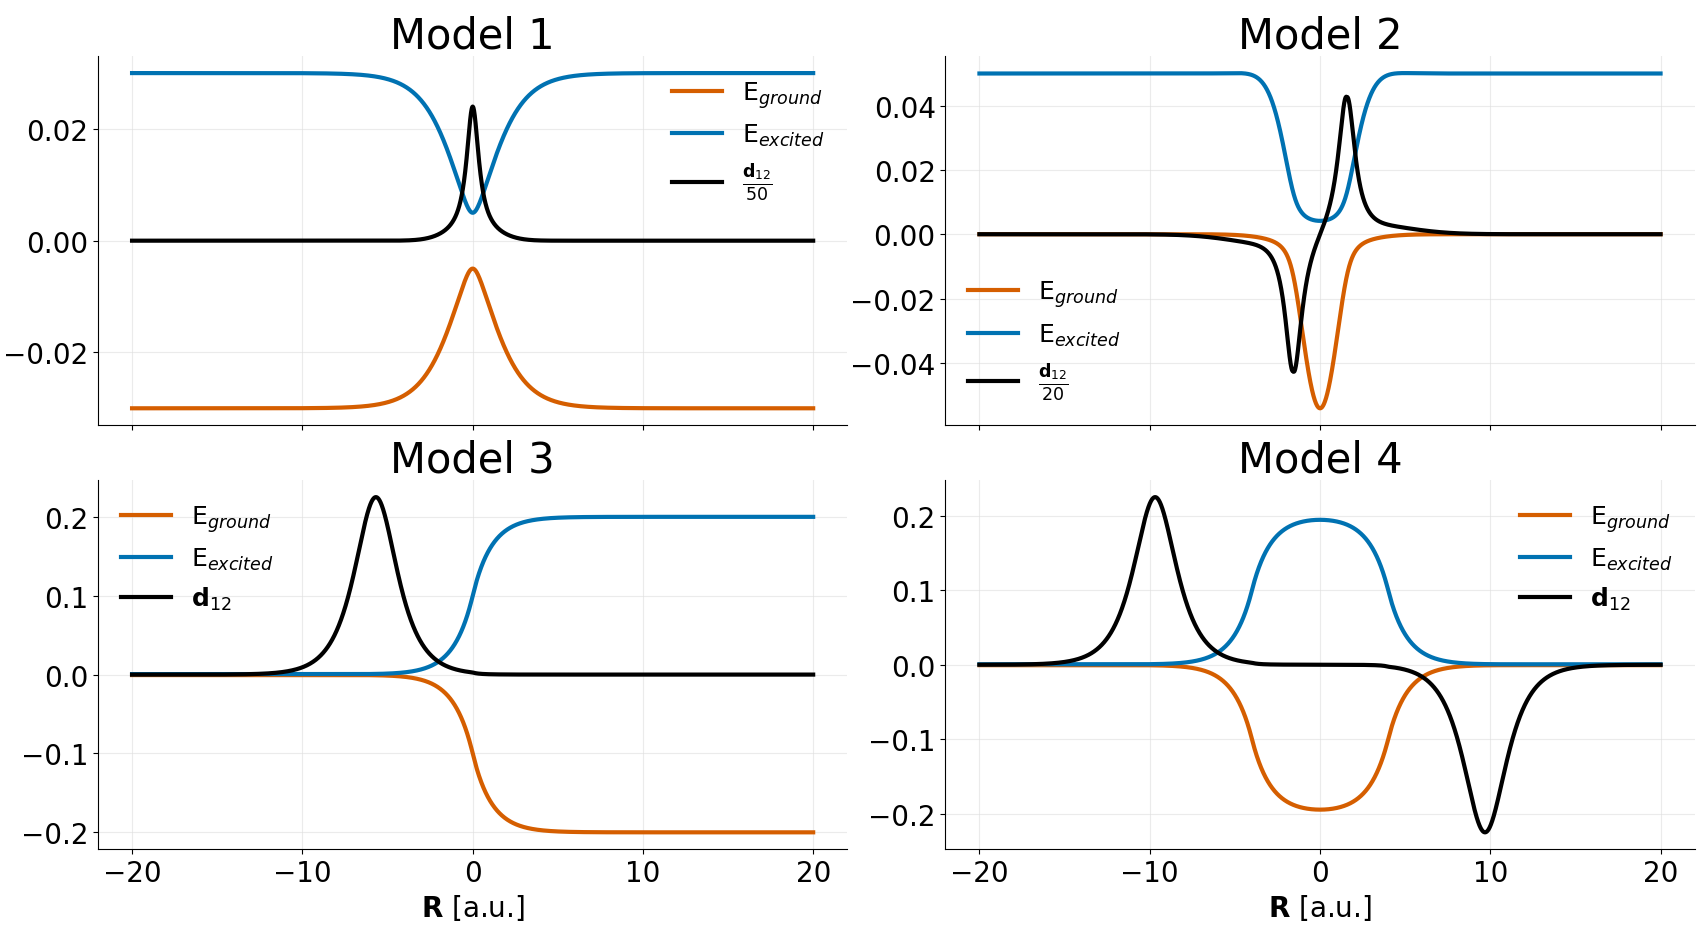
\includegraphics[width=\textwidth]{Chapter_tullyModels/model_schematics.png}
  \caption{\label{fig:tully_schematics}Adiabatic potential energy surfaces (orange and blue) and element 1, 2 of the nonadiabatic coupling vector (black) for the 4 model systems. For parameters see appendix \ref{app:tully_params}.}
\end{figure}
\newpage
\noindent In order to initialise the simulations coordinates and velocities were sampled from the Wigner phase-space distribution of a gaussian nuclear wavepackets given by equation \eqref{eq:initial_nucl_wp}. A derivation of this can be found in appendix \ref{app:Wigner}. The nuclear positions/velocities were then propagated using a velocity verlet algorithm and the adiabatic expansion coefficients were propagated using a 4$^{th}$ order Runge-Kutta method.
\begin{equation}
  \chi(R, 0) = \frac{1}{(\pi \mu^2)^{\frac{1}{4}}} e^{-\frac{(R - R_0)^2}{2 \mu^2} + \im k_0 (R - R_0) }
  \label{eq:initial_nucl_wp}
\end{equation}
The adiabatic coefficients were initialised purely on the ground state and the initial width of the nuclear wavepacket was set to $\mu = \sqrt{2}$ bohr. 2 values of initial momenta $k_0$ were chosen for each model, 1 low value and another higher one. Full details of all input parameters can be found in appendix \ref{app:tully_params}. I have implemented a serial version of CTMQC acting on Tully's toy model systems and real molecular systems using couplings derived from the analytic overlap method \cite{gajdos_ultrafast_2014} within the software package CP2K \cite{cp2k} and for Tully's model systems as standalone python code. These are accessible publicly via github repositories at: \href{https://github.com/95ellismle}{github.com/95ellismle}. This work will only focus on results from the CP2K implementation as we will later see this code extended and applied to systems of real Ethylene molecules.

\section{Testing My Implementation}
The motivation behind implementing CTMQC for the Tully models was to serve as a verifiable base for later extensions, such as integrating CTMQC within the fragment-orbital based (FOB) \cite{spencer_fob-sh:_2016} framework which will be discussed in a later chapter \cite{chap:molecular_systems}. Using such simple systems will also help to clarify how each new parameter works and make testing and debugging easier. As well as many numerical tests on individual terms in the equations,  I have implemented some physical tests on the overall system dynamics. In this section, I will outline the key tests I have performed on both the Ehrenfest and full CTMQC parts of the equations. These are: ... %verifying we obtain Rabi oscillation in the limit of fixed nuclear geometries, checking energy and the norm of the wavefunction is conserved and verifying the time-derivative of the sum over trajectories of adiabatic populations is 0.
\\\\
%\subsection{Rabi Oscillation}
%Rabi Oscillation is a solution of the time-independent Schr\"odinger equation and occurs when nuclear coordinates are fixed in place while electronic coordinates aren't. Some information is given in appendix \ref{ap:Rabi}. This can be used to test the Runge-Kutta propagator as Rabi Oscillation should be observed when velocities are set to 0.
\subsection{Comparisons To Literature}
There have been 2 papers published applying CTMQC to the Tully models \cite{gossel_coupled-trajectory_2018, agostini_quantum-classical_2016} and both contain results for the 4 Tully models shown in fig \ref{fig:tully_schematics}. The results contain data on the (ground state) adiabatic populations and a coherence indicator as shown in equation \eqref{eq:coherence_indicator} for 16 different simulations (a low and high initial momentum simulation of Models 1, 2, 3 and 4). 
\begin{equation}
	|\rho_{12}(t)|^2 = \frac{1}{N_{tr}} \sum_{I=1}^{N_{tr}} |C_{1}^{(I)}(t)|^2 |C_{2}^{(I)}(t)|^2
	\label{eq:coherence_indicator}
\end{equation}
\\\\
In order to compare to results in the literature the same setup had to be used. In this case this meant sampling individual trajectory initial conditions (positions and momenta) from a Wigner distribution with a mean position and momenta given in appendix \ref{app:tully_params}. The wavefunction was initialised purely on the ground state and the same integrator was used for the nuclear and electronic propagation (velocity verlet and RK4 respectively).
\subsection{Ehrenfest}
\begin{figure}[h]
	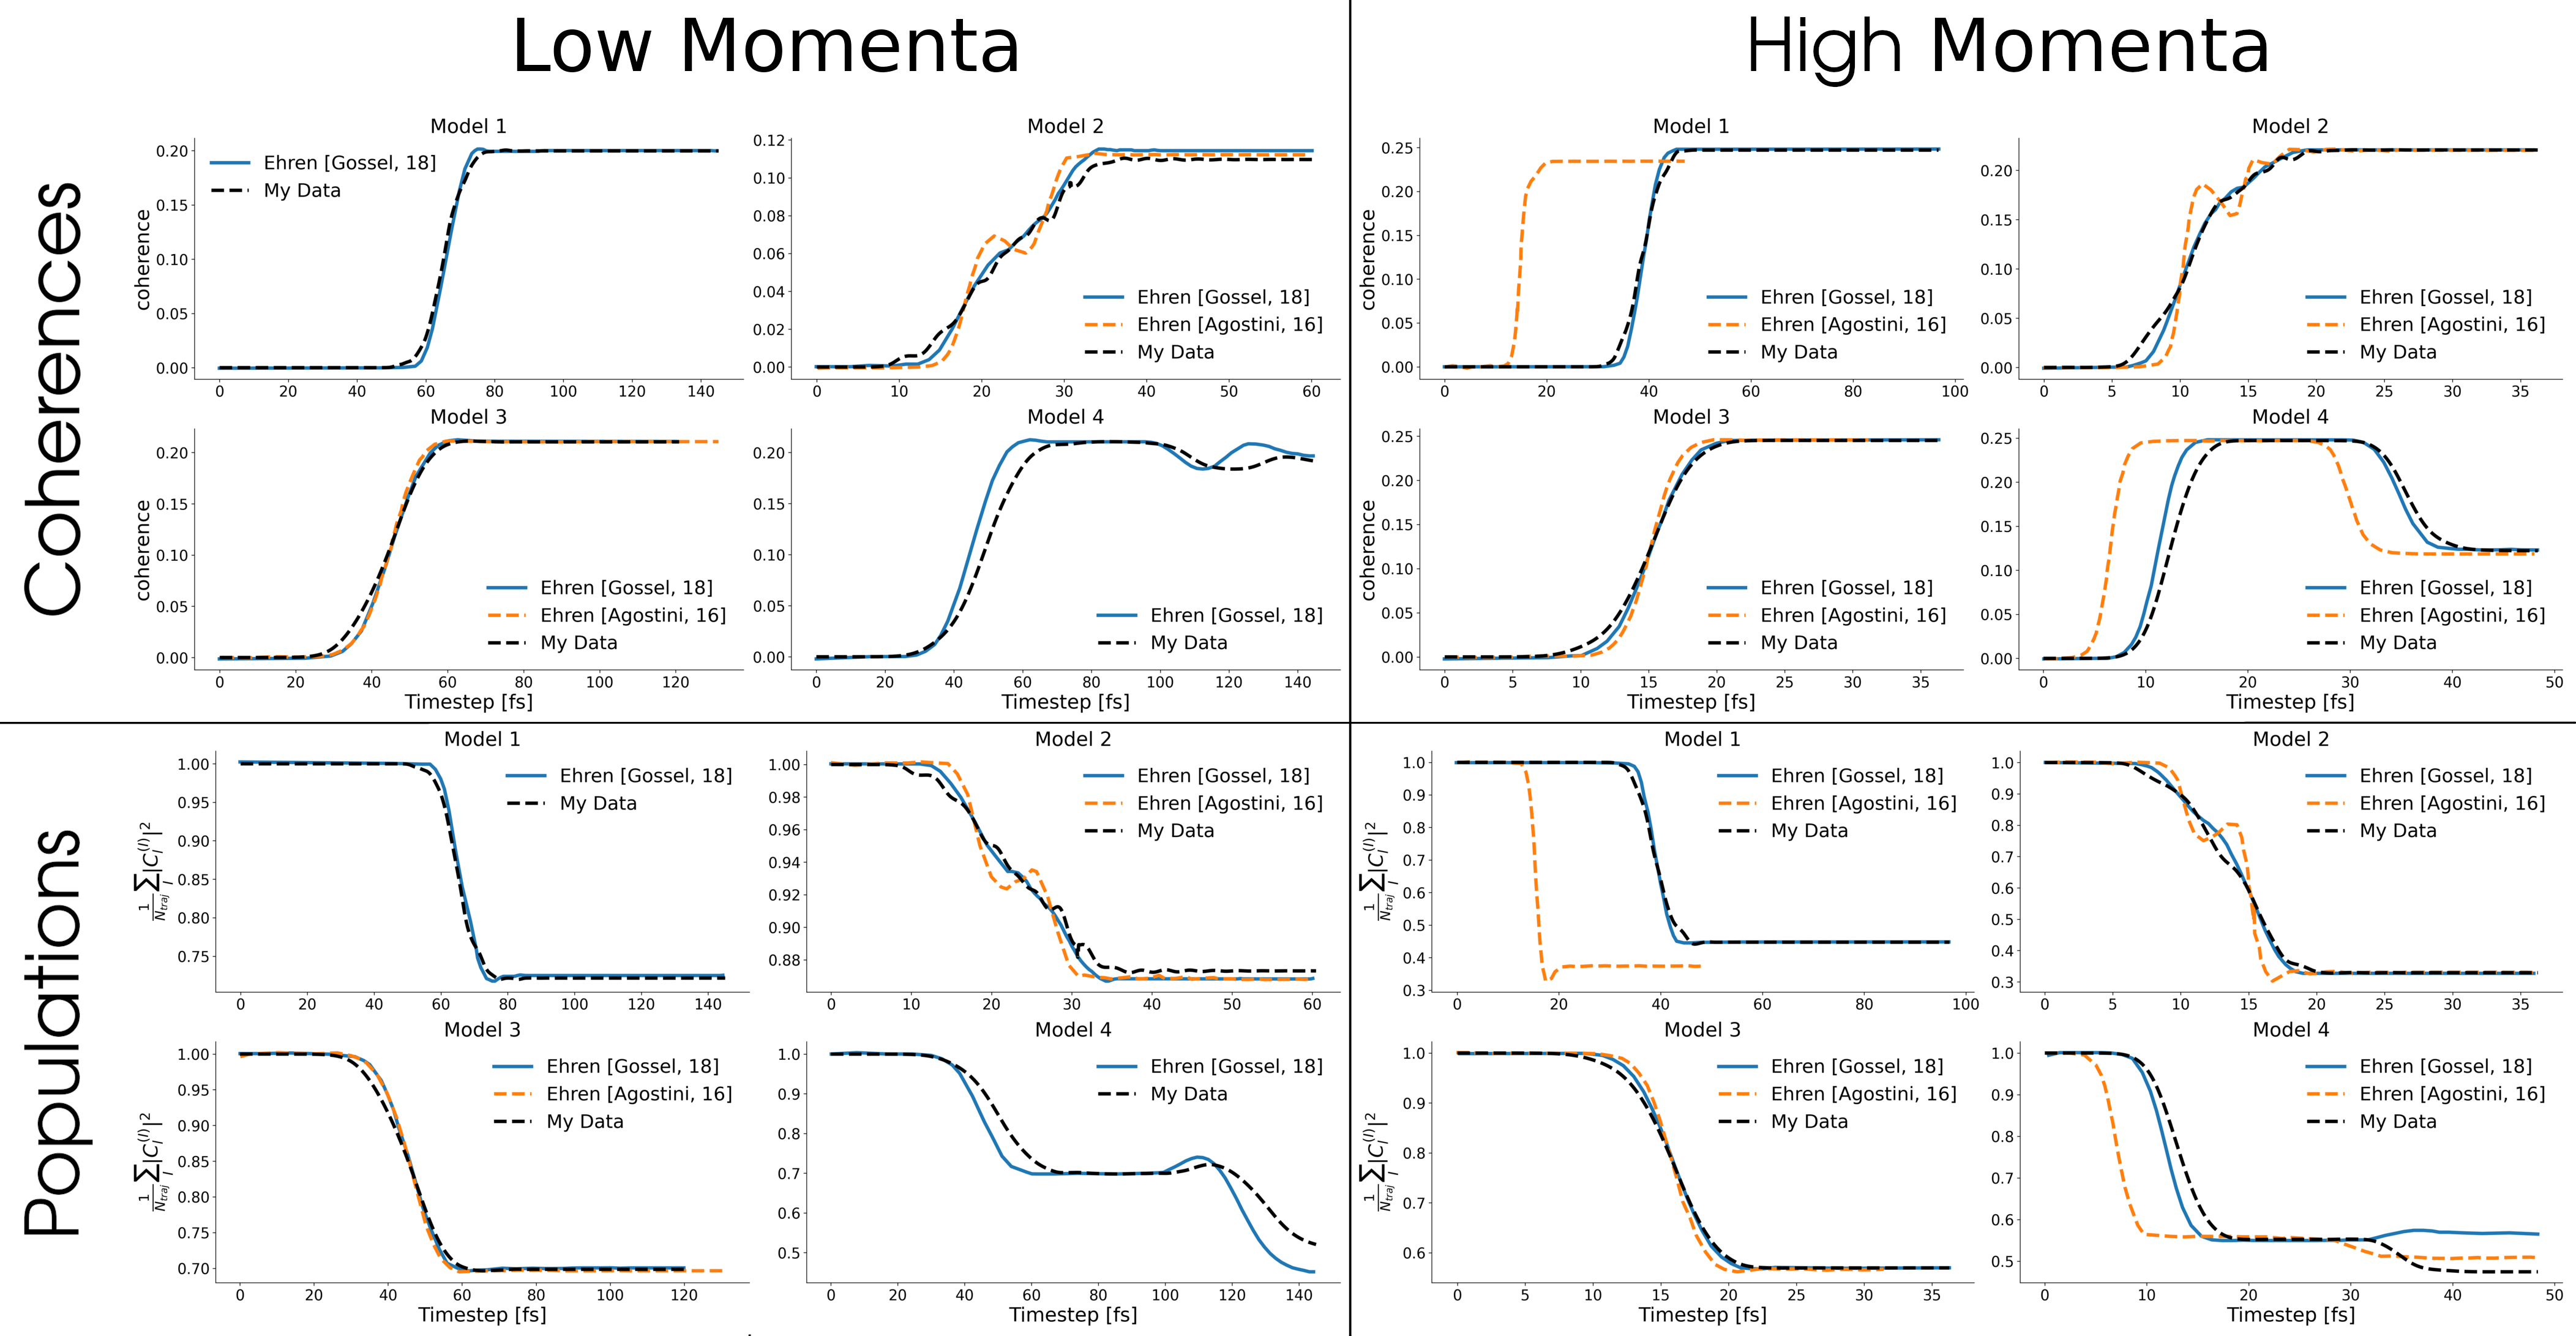
\includegraphics[width=\textwidth]{img/CTMQC/TullyModels/Ehren_LitComp.png}
	\caption{\label{fig:LitCompEhrenTully}A comparison of my implementation of Ehrenfest (for 4 model Hamiltonians) and results from the literature. The black dashed lines show my data (ground state ad pops), the orange dashed lines are data from Agostini, 16 \cite{agostini_quantum-classical_2016} and the blue solid lines are from Gossel, 18 \cite{gossel_coupled-trajectory_2018}. The figures are labelled with their model number, whether the initial momentum was high or low and whether the populations or coherence indicator was plotted.}
\end{figure}
\noindent My results as well as the relevant data taken from Agostini, 16 and Gossel, 18 \cite{agostini_quantum-classical_2016, gossel_coupled-trajectory_2018} are shown in figure \ref{fig:LitCompEhrenTully} for Ehrenfest dynamics. This is equivalent to full CTMQC dynamics where the quantum momentum term is set to 0. Hence, we can test most parts of the code (i.e. Runge-Kutta propagation, velocity verlet, inputs, force calculations etc...) while ignoring the new quantum momentum and accumulated adiabatic force terms.
\\\\
The results in figure \ref{fig:LitCompEhrenTully} show that both the adiabatic populations and coherence indicator give exactly the same results as in the literature, within reasonable error. Any deviations of results come from either a slightly different initial sampling of positions (sampled from a Wigner distribution) or small errors in retrieving data from the graphs in each paper. For example, in the case of the high initial momentum simulation of model 4 all 3 results show some differences though the trend is very similar. This is true also in the Model 2 results where the Agostini, 16 populations show some transient oscillations before settling onto the same equilibrium population. This may be due to a smaller spread of positions being used in the initial sample leading to similar oscillations that aren't smoothed out in the averaging over all trajectories. There are also a couple of models that start at a slightly different initial mean position in Frederica, 16 thus they hit the nonadiabatic crossing region sooner. These are model 1 and 4 for the high momentum case.
\\\\
Although not all results are exactly the same, I believe the populations agree well enough within a reasonable error to serve as a confirmation of my implementation.
\subsubsection{Comparisons of Ehrenfest to Other Data}
In a Subotnik, 2010 \cite{SubotnikMomentumEhrenfest}, results were published for Ehrenfest simulations carried out on the 3 original Tully Models. In that work, the author presented the probabilities of the population being found transmitted through the region of nonadiabatic coupling on the ground or excited state and the probability of being reflected on the ground or upper state. In the results below, I will show comparisons of just the transmission probability onto the ground state. That is, the population that travels on the ground state beyond the region of high nonadiabatic coupling. Other probabilities will not be shown in the interest of brevity, though they agree with the published results as well as the ground state transmission in figure \ref{fig:SubotnikComparison}.
\begin{figure}[h]
  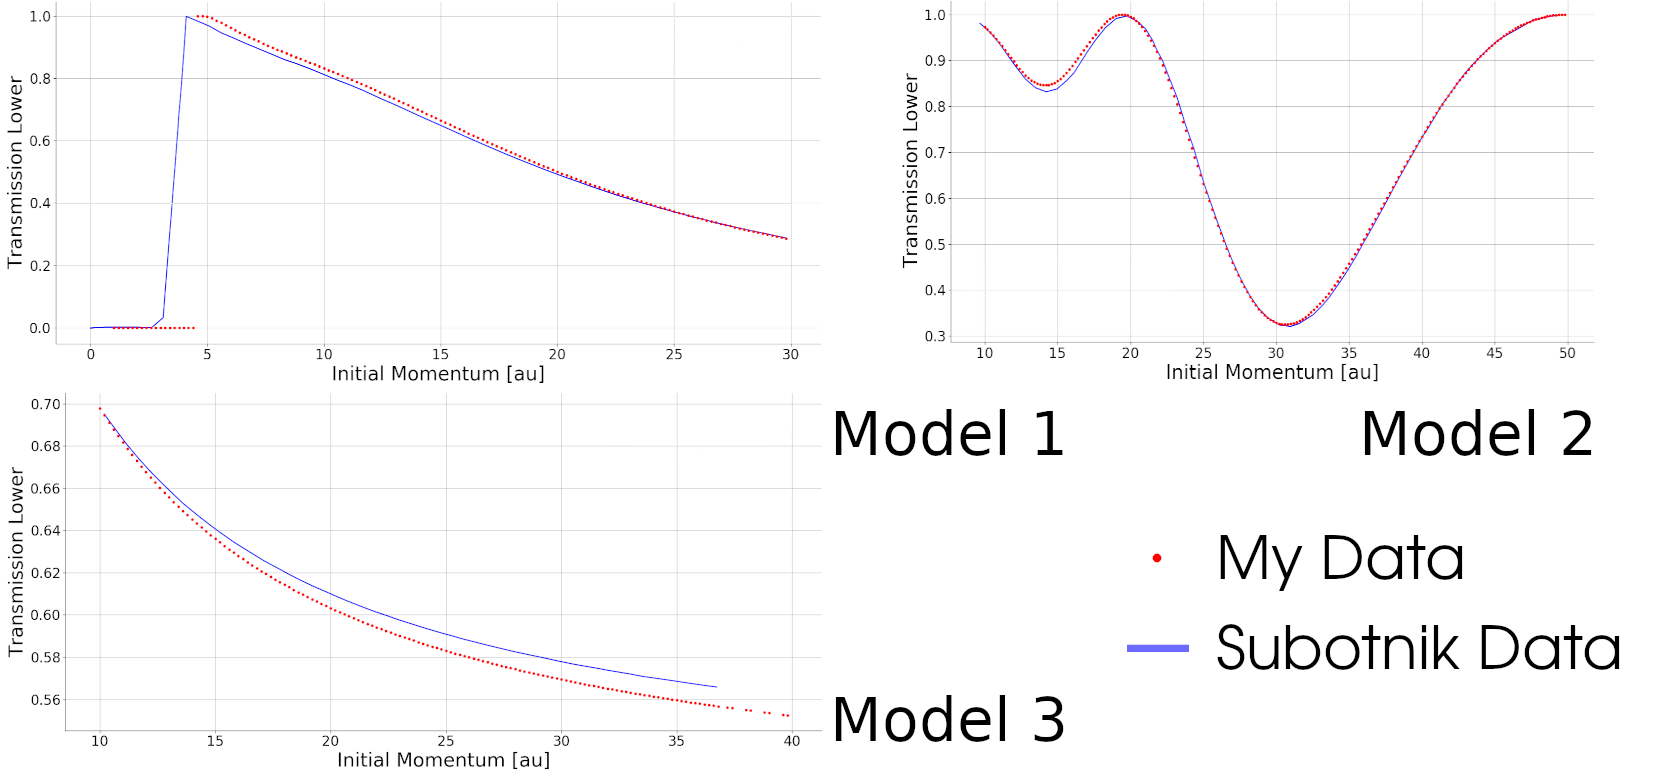
\includegraphics[width=\textwidth]{img/CTMQC/TullyModels/Ehrenfest_vs_Subotnik.png}
  \caption{\label{fig:SubotnikComparison}Comparison of transmission probabilities through the region of high nonadiabatic coupling on the ground state. Tully model 1 is shown in the top-left, Tully model 2 is shown in the top-right and Tully model 3 is shown in the bottom-left.}
\end{figure}
\\
As can  be seen in figure \ref{fig:SubotnikComparison} my implementation of the Ehrenfest simulation code for the Tully models agrees very well with those in Subotnik, 2010 \cite{SubotnikMomentumEhrenfest}. The small deviation (less than 1\% disagreement) within each model is due to errors in retrieving data from images in original paper.
\subsection{CTMQC}
\begin{figure}[h]
	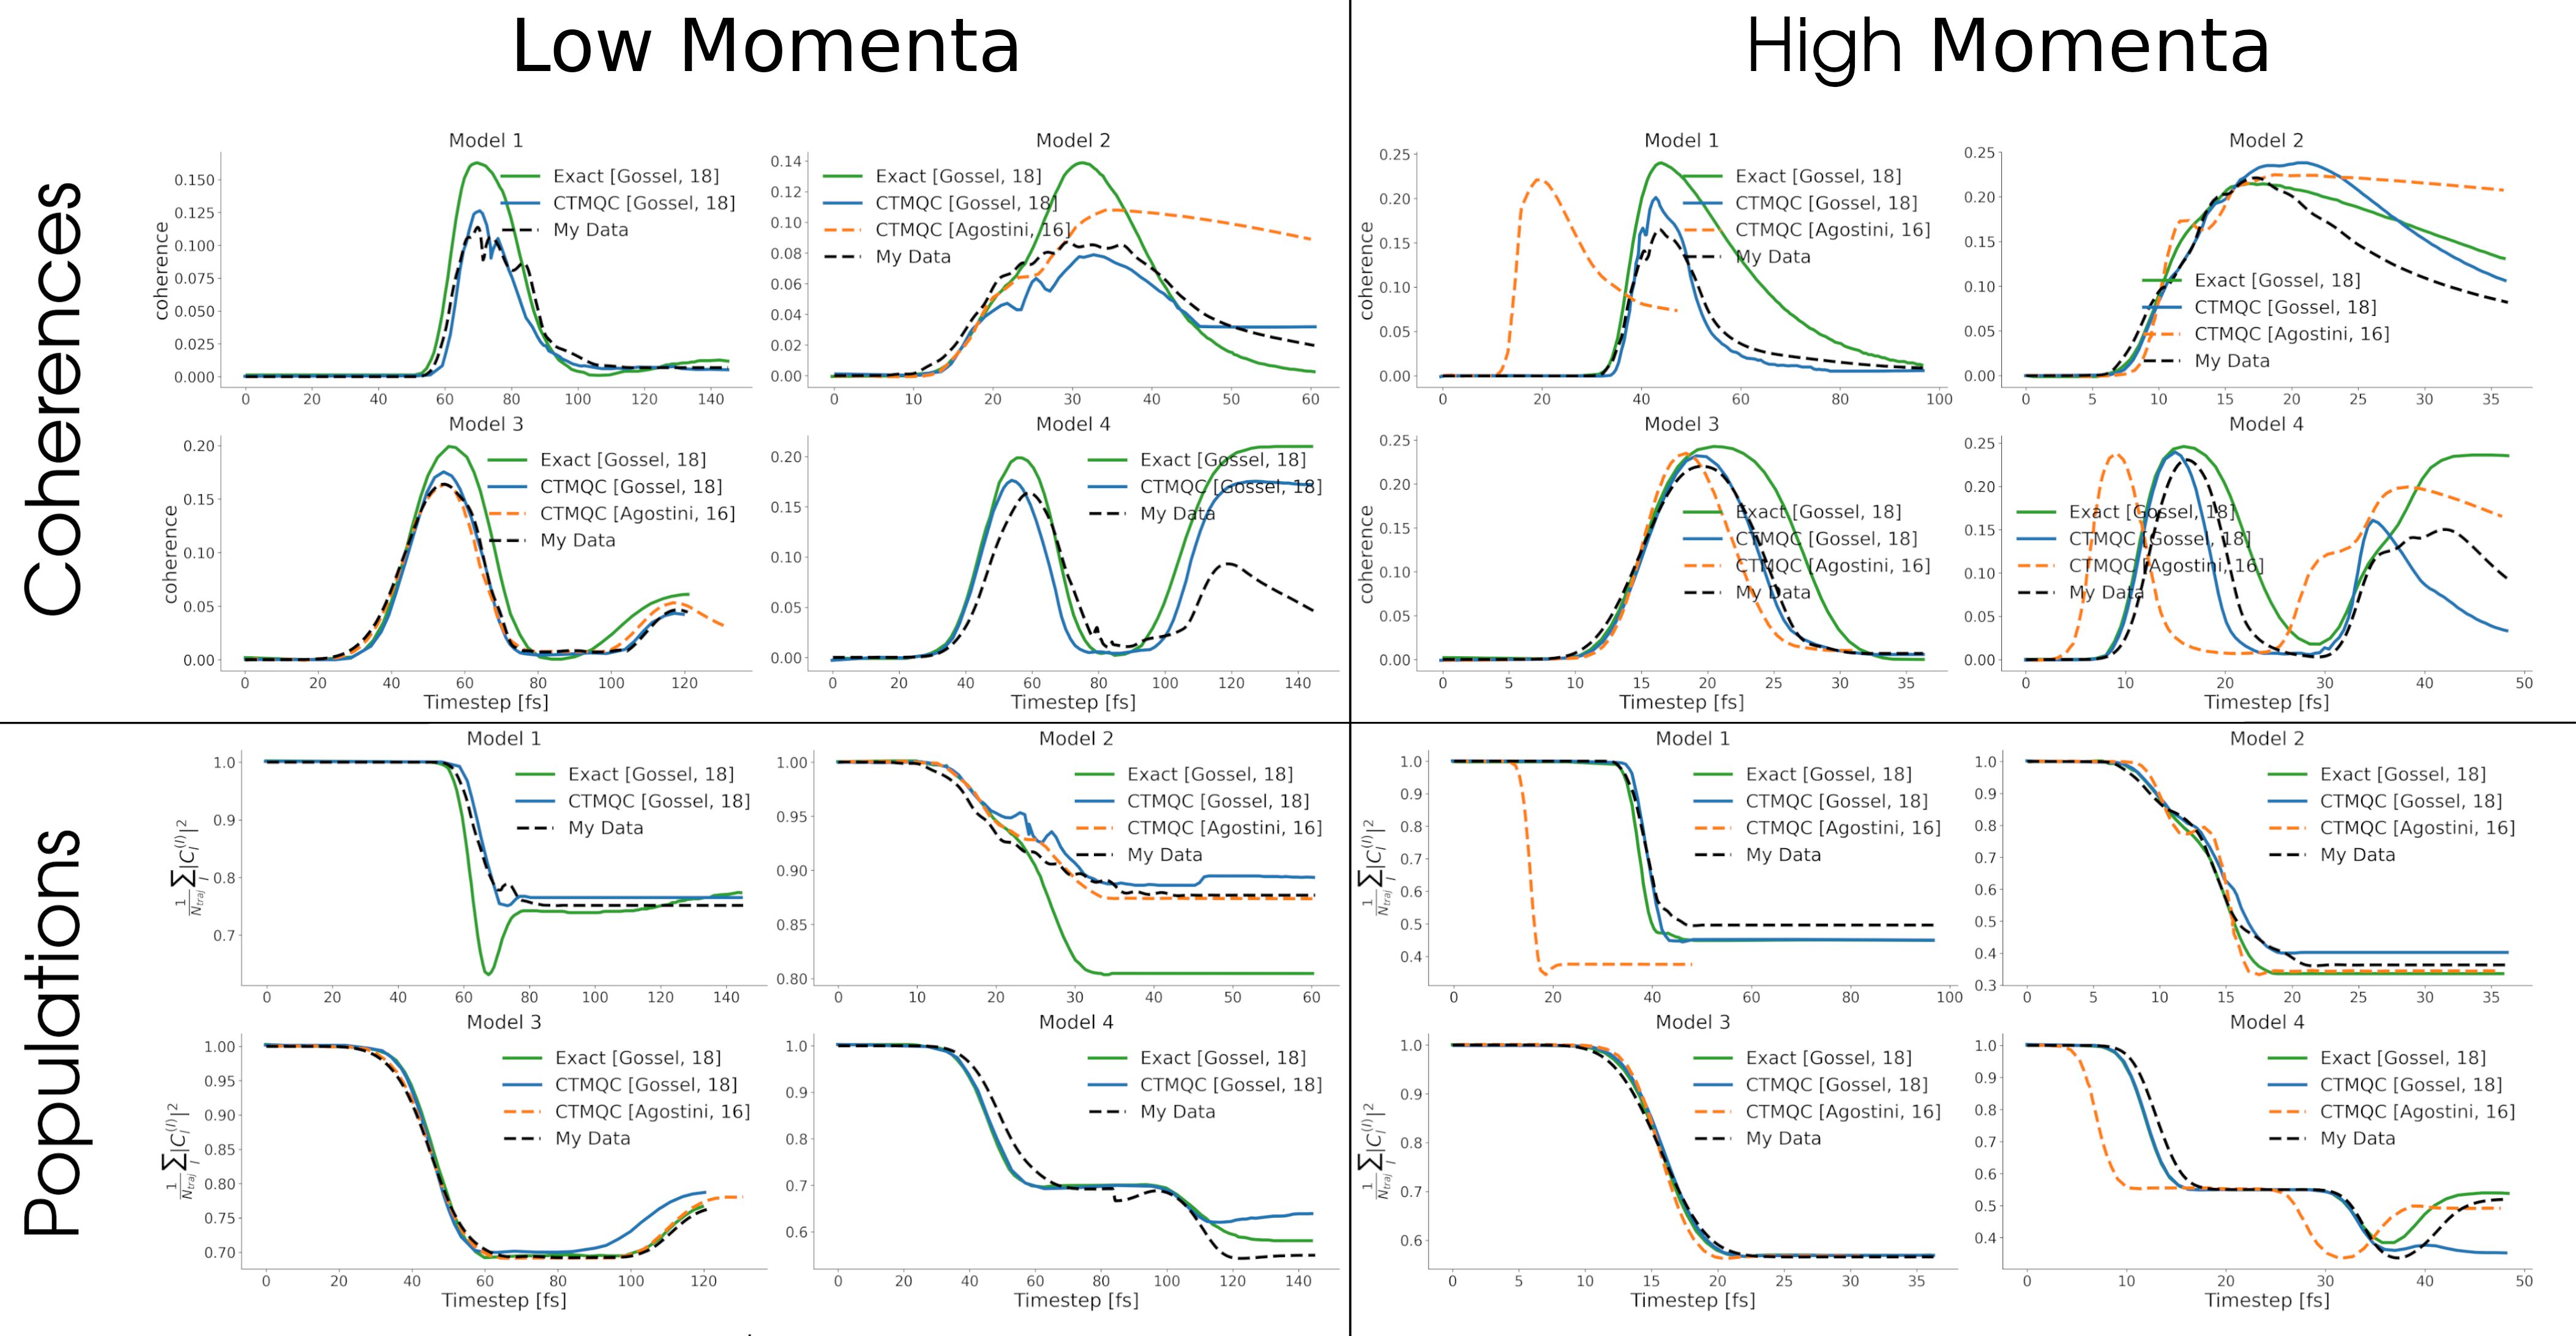
\includegraphics[width=\textwidth]{img/CTMQC/TullyModels/CTMQC_LitComp.png}
	\caption{\label{fig:LitCompCTMQCTully}A comparison of my implementation of full CTMQC (for 4 model Hamiltonians) and results from the literature. The black dashed lines show my CTMQC data (ground state ad pops), the orange dashed lines are data from Agostini, 16 \cite{agostini_quantum-classical_2016} and the blue solid lines are from Gossel, 18 \cite{gossel_coupled-trajectory_2018}. The solid green line shows data from exact quantum mechanical simulations given in Gossel, 18. The figures are labelled with their model number, whether the initial momentum was high or low and whether the populations or coherence indicator was plotted.}
\end{figure}
To test the full CTMQC equations I now turn on the quantum momentum ($\mathcal{Q}_{lk, \nu}^{(I)}$) and accumulated adiabatic force ($\mathbf{f}_{l, \nu}^{(I)}$) terms. These provide the extra decoherence that is missing in the standard Ehrenfest representation and allow populations of individual trajectories to collapse onto a single adiabatic state. Without these terms (e.g. in Ehrenfest dynamics) all trajectories follow the same mean potential energy surface and detailed balance is not conserved.
\\\\
The results for my implementation are given in figure \ref{fig:LitCompCTMQCTully}. This time, unlike in the Ehrenfest code, we see some major discrepancies between the 3 results. These cannot solely be explained as small errors from slightly different sampling of initial positions. We can see that the errors mainly appear in the coherence indicator, looking at the bottom row in figure \ref{fig:LitCompCTMQCTully} it appears that both the Agostini and Gossel results match mine (in dashed black line) very closely. The largest difference is seen in model 4, high momentum where the Gossel data and mine follow a similar trend and the Agostini data follows the exact curve more closely. However, looking at the coherence indicators in the above row we see a different story. My data tends to follow the Gossel data fairly closely, while the Agostini data follows a different pattern. This is due to differing parameters being used to calculate the quantum momentum term.
\\\\
To calculate the quantum momentum one must take the spatial derivative of the nuclear density. However, the nuclei are classical and represented by a point. In order to calculate the nuclear density the procedure outlined in the supplementary information of Min, 17 \cite{min_ab_2017} was to smear out the nuclear density by describing each classical atom with a gaussian distribution of width $\sigma$ and mean $\mathbf{R}^{(I)}_{\nu}(t)$ (i.e. the atomic position). The method for determining the parameter $\sigma$ has not been outlined therefore it is very hard to develop a method to exactly reproduce the results found in the 2 CTMQC papers. In figure \ref{fig:LitCompCTMQCTully} a constant sigma of $\sigma = 0.35$ bohr was taken to closely match the Gossel, 18 data. The fact that the curves match in many cases almost exactly makes me think this was the method employed in Gossel, 18 too. It also serves as a confirmation of the full implementation of CTMQC.


\subsection{Norm Conservation}
\label{sect:normCons}
\begin{figure}[h]
	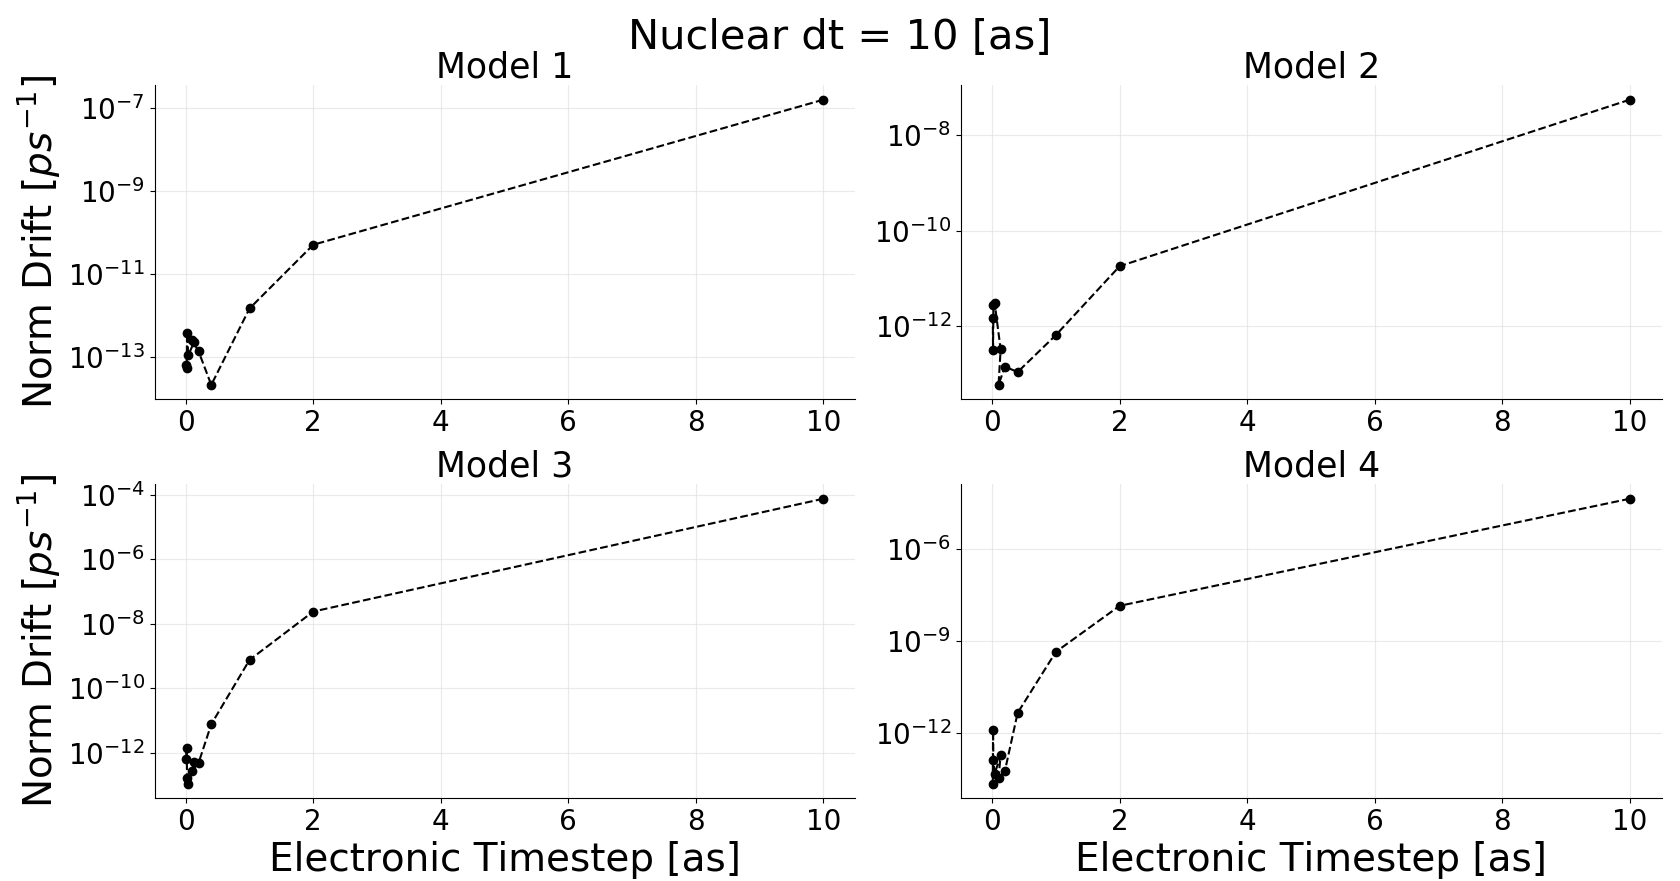
\includegraphics[width=\textwidth]{/home/matt/Documents/PhD/PhD_Thesis/img/CTMQC/TullyModels/Ehren_Norm_Conservation.png}
	\caption{\label{fig:EhrenNormCons}The norm conservation averaged over all replicas for Ehrenfest simulations with various electronic timesteps for each Tully model using a initial high momenta.}
\end{figure}

\noindent In appendix \ref{ap:norm_cons}, it is shown that the norm of the adiabatic expansion coefficients should be conserved throughout the simulation. In order to test this simulations were carried out using the parameters from the high momentum cases given in appendix \ref{app:tully_params} with various size electronic timesteps (i.e. the timestep used to propagate the electronic subsystem). The nuclear timestep was held constant. As can be seen in figure \ref{fig:EhrenNormCons}, the norm of the wavefunction is conserved within numerical error ($10^{-12}$) when using a sufficiently small timestep in every Tully model. However, when we now use the full CTMQC equation we see a very different picture.
\begin{figure}[h]
	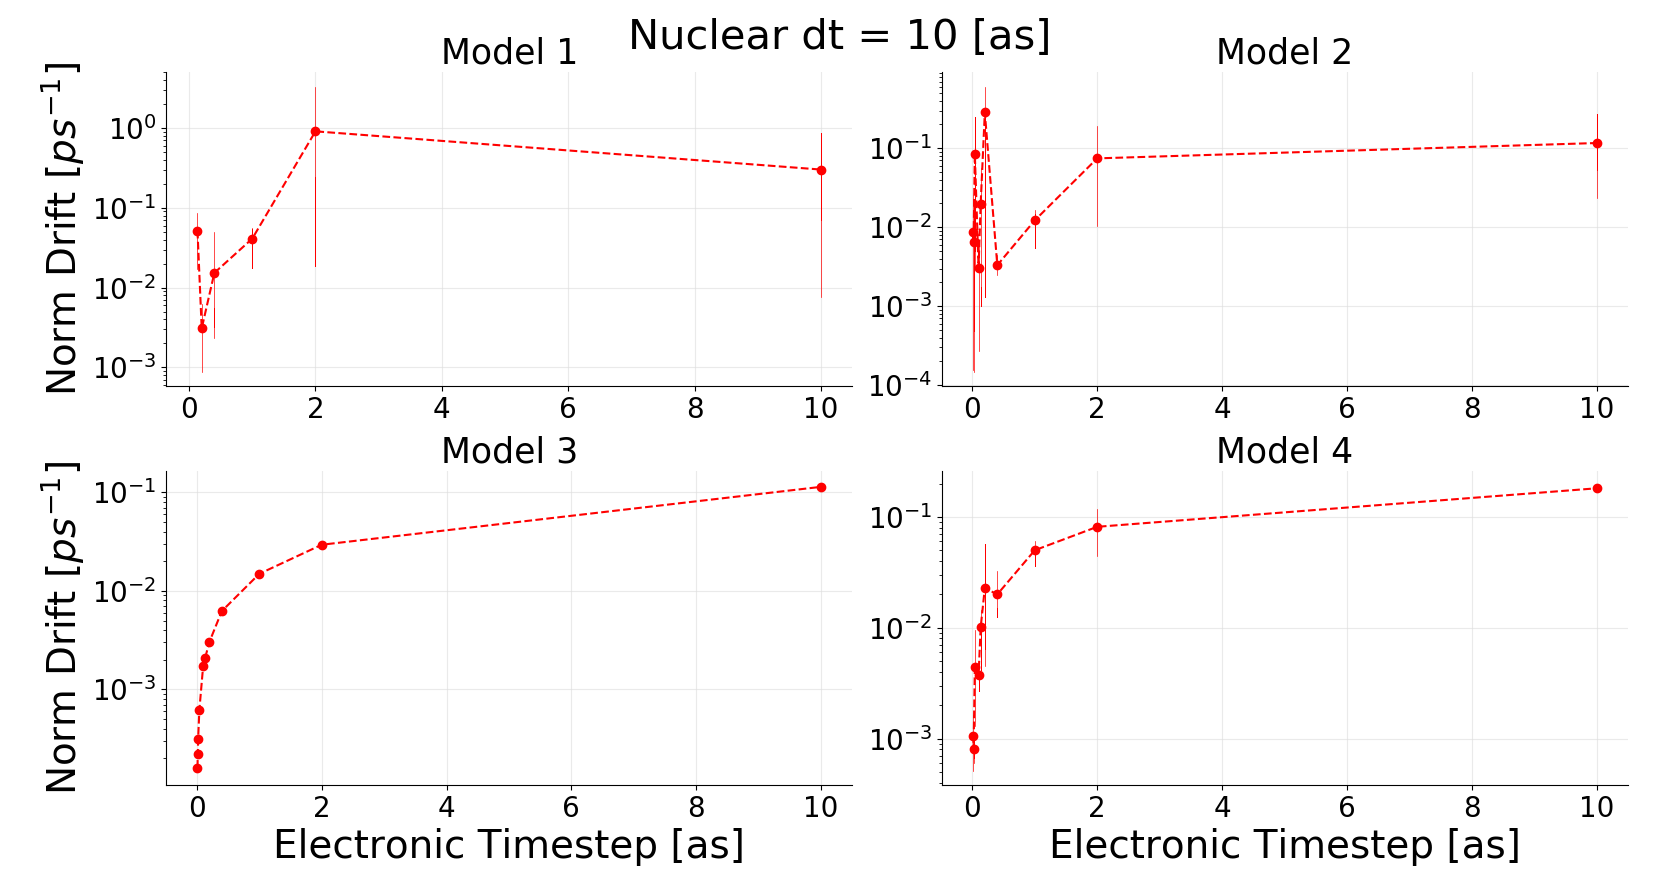
\includegraphics[width=\textwidth]{/home/matt/Documents/PhD/PhD_Thesis/img/CTMQC/TullyModels/CTMQC_Norm_Conservation.png}
	\caption{\label{fig:CTMQCNormCons}The norm conservation when using standard CTMQC as outlined in the literature for each of the Tully models. These simulations were ran with a high initial momentum. The red markers show data points and vertical bars show error bars associated with each point.}
\end{figure}
\\
In figure \ref{fig:CTMQCNormCons}, we can see that only in Model 3 we see a similar trend as in Ehrenfest for the norm conservation -i.e. a decreasing electronic timestep gives a rapidly decreasing norm drift. In models 1 and 2 we see that the norm drift doesn't get much better as we decrease the timestep and there are large error bars associated with each data point. In model 4 this is less pronounced but is still clearly effected. This is due to an instability in the way the quantum momentum term ($\mathcal{Q}_{lk, \nu}^{(I)}$) is calculated.
\\\\
The calculation of the quantum momentum is discussed in detail in Min, 17 \cite{min_ab_2017} and outlined in the introduction to the thesis in section \ref{sect:QM_Calc}. As mentioned in that section, the denominator in the expression for $\mathbf{R}_{lk, \nu}$ may be positive or negative and when it switches between the 2 it can approach zero very closely. If this denominator approaches zero more quickly that the numerator then we can see large spikes in the $\mathbf{R}_{lk, \nu}$ term which can lead to large norm drifts.

\subsubsection{Quantum Momentum Instabilities}
\label{sect:QlkSpikes}
\begin{figure}[h]
	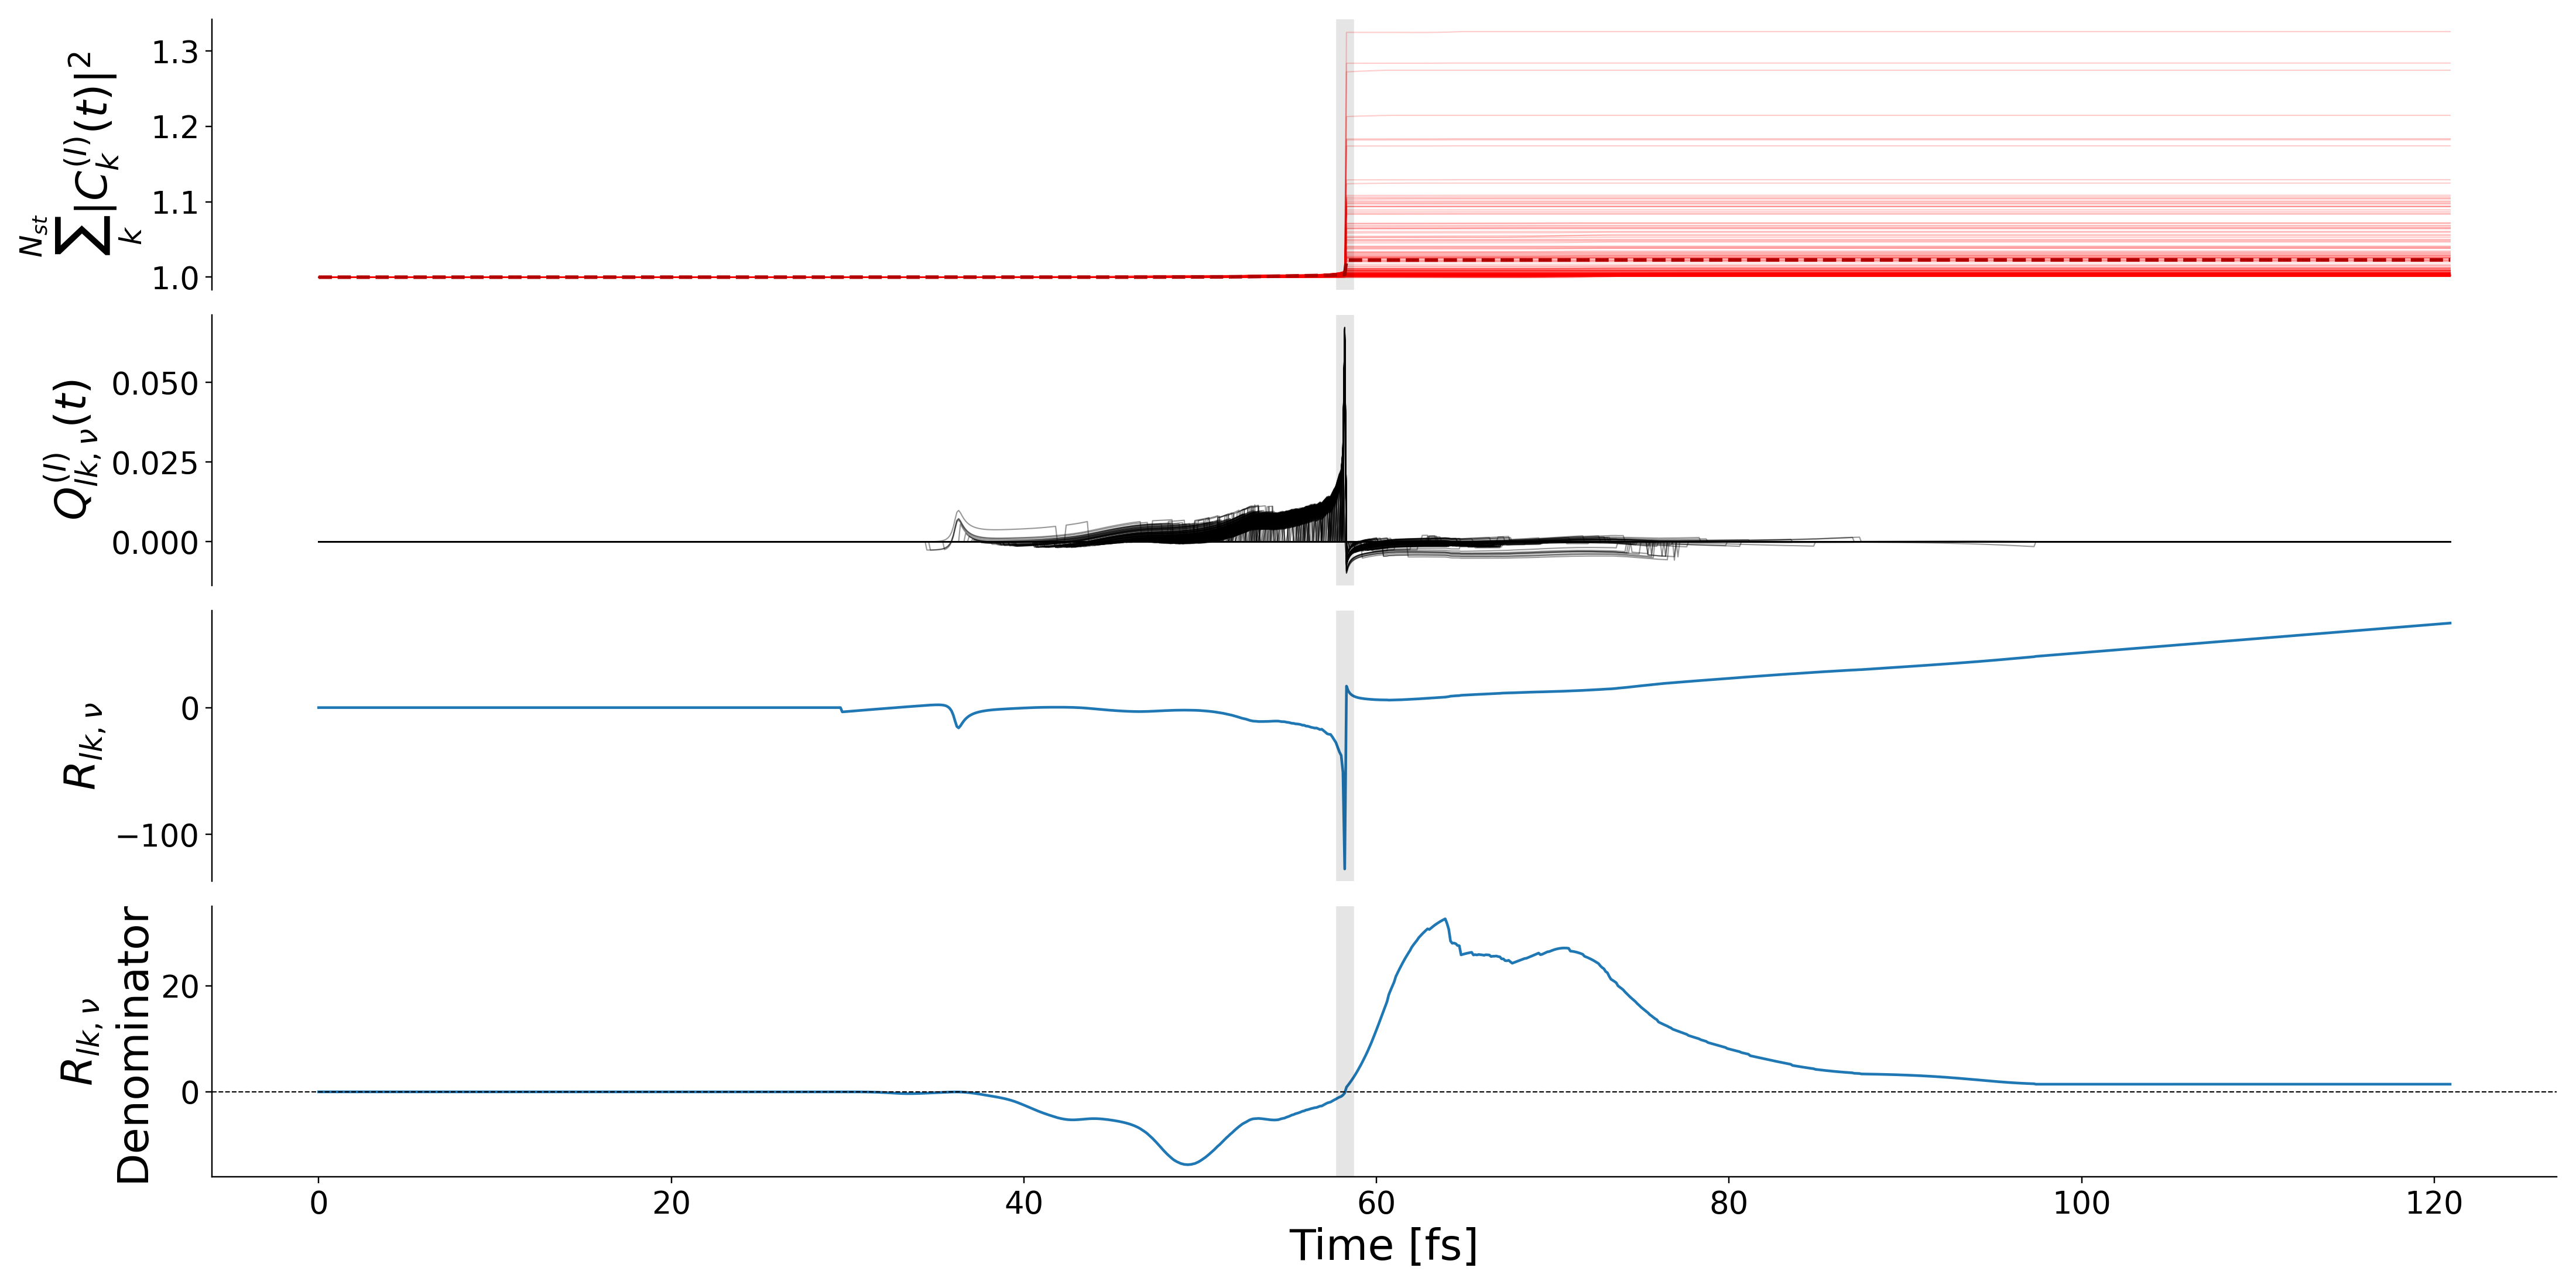
\includegraphics[width=\textwidth]{./img/CTMQC/TullyModels/Spikes/RlkDenom_Rlk_Qlk_Norm.png}
	\caption{\label{fig:QlkSpike}As the denominator of the $\mathbf{R}_{lk,\nu}$ term approaches zero (bottom panel) the full $\mathbf{R}_{lk, \nu}$ term (2$^{\text{nd}}$ to bottom panel) can approach infinity which propagates through the $\mathcal{Q}_{lk, \nu}^{(I)}$ term (2$^{\text{nd}}$ to top panel) causing discontinuities and norm drift in the populations (top panel). The grey vertical bar denotes the region the denominator approaches 0. The thin solid red lines in the top panel show the norm drift for individual trajectories.}
\end{figure}
\noindent As we can see in figure \ref{fig:QlkSpike}, as the denominator of the $\mathbf{R}_{lk, \nu}$ term approaches 0 the full $\mathbf{R}_{lk, \nu}$ term may spike causing a discontinuity in the populations. The reason this only occurs in Models 1, 2 and 4 is due to the fact that the difference in the adiabatic momenta terms ($\mathbf{f}_{l, \nu}^{(I)} - \mathbf{f}_{k, \nu}^{(I)}$) doesn't cross 0 in Model 3. In order to correct for this I have investigated a number of corrections to the calculation of the quantum momentum. These depend on the detection of the spikes/divergences in the $\mathbf{R}_{lk, \nu}$ term and then the appropriate treatment of them. In order to detect the divergences a simple threshold on the $|\frac{\delta}{\delta t} \mathbf{R}_{lk, \nu}|$ is applied when the denominator of the $\mathbf{R}_{lk, \nu}$ is sufficiently close to 0. For example, if the absolute time-derivative of the $\mathbf{R}{lk, \nu}$ term is larger than a value (say 5) and the bottom of the fraction in equation \eqref{eq:Rlk} is within 0.1 of 0 then we assume the $\mathbf{R}_{lk, \nu}$ term is diverging and the simulation code then uses a different method of propagating the electronic coefficients.
\clearpage
\noindent The alternative propagation methods I have investigated are:
\begin{enumerate}
	\item Use Ehrenfest Dynamics (set $\mathcal{Q}_{lk, \nu}$ term to 0).
	\item Extrapolate the value of $\mathbf{R}_{lk, \nu}$ from values before the divergence (see appendix \ref{ap:RlkExtrap}).
	\item Switch to using the alternative intercept $\mathbf{R}_{0, \nu}^{(I)}$ (see appendix \ref{ap:AltIntercept}).
\end{enumerate}
of these 3 methods, method 3 was the most successful in reducing the norm drift in the Tully Models as can be seen in figure \ref{fig:NormConsCorr}.
\begin{figure}[h]
	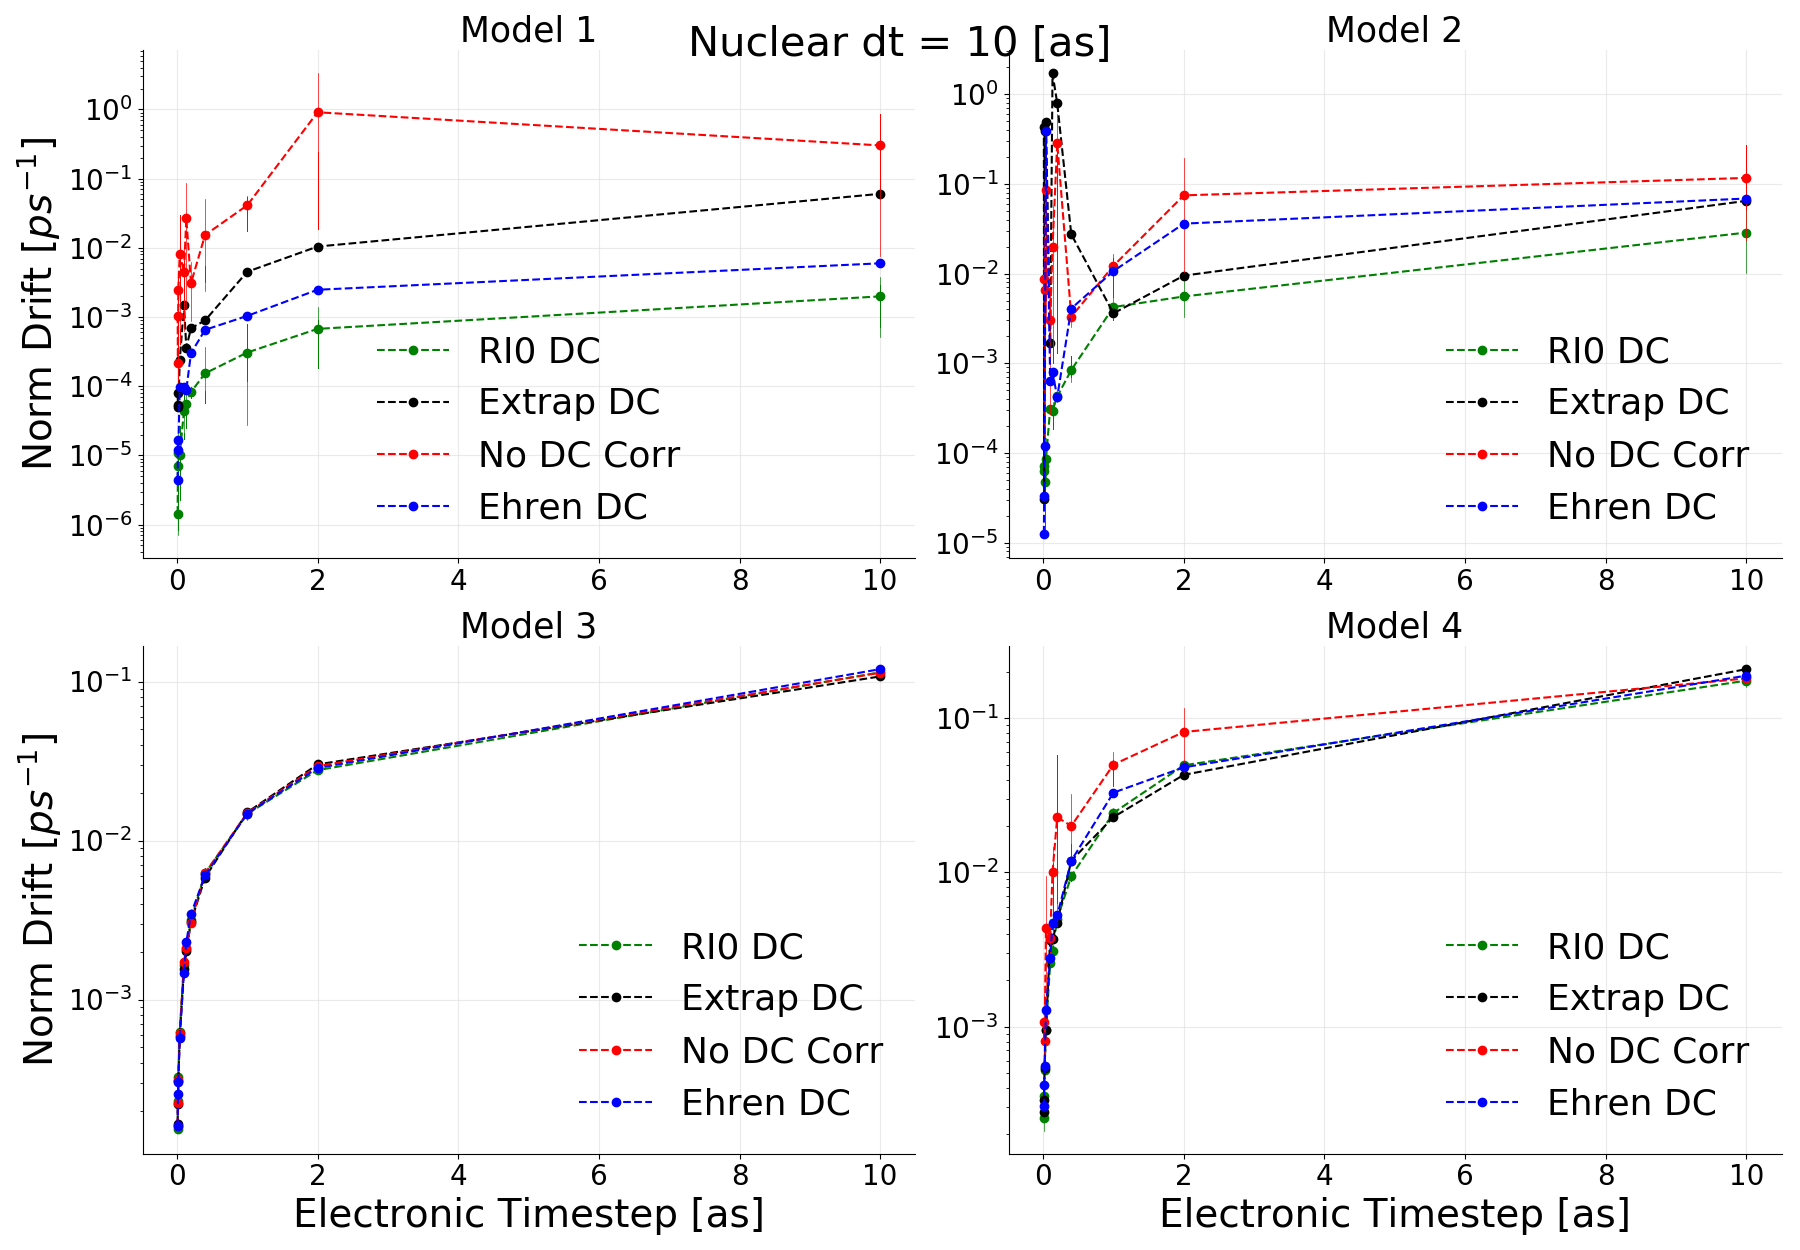
\includegraphics[width=\textwidth]{img/CTMQC/TullyModels/CTMQC_Norm_Conservation_wCorr.png}
	\caption{\label{fig:NormConsCorr}Norm conservation in CTMQC after applying a divergence correction to the $\mathbf{R}_{lk, \nu}$ term. RI0 refers to method 3, Extrap DC refers to method 2 and Ehren DC refers to method 1. No DC Corr shows the population norm without any corrections applied.}
\end{figure}
In figure \ref{fig:NormConsCorr} we see the norm drift results after the 3 $\mathbf{R}_{lk, \nu}$ correction methods have been applied. The red curve shows the original data (as in figure \ref{fig:CTMQCNormCons}) with it's large divergences in the norm drift. The green curve shows the alternative intercept method, the blue curve shows the effect of switching to Ehrenfest during the $\mathcal{Q}_{lk, \nu}^{(I)}$ spikes and the black shows a method that involved extrapolating the $\mathbf{R}_{lk, \nu}$ value from data before the spike began. We can see clearly all 3 methods improve the norm drift, though using the alternative intercept seems to help the most. Model 3 is not affected as we do not see these divergences in the $\mathbf{R}_{lk, \nu}$ due to the denominator in this particular model never crossing from positive to negative (through zero). It is important to note that in each of the models with the divergence correction applied all models exhibit the expected trend of decreasing the time-step improves norm conservation. However, the norm conservation in all 4 models is still significantly higher ($\sim$ 7-8 orders of magnitude) higher than that of Ehrenfest. I think this is due to the product of the adiabatic populations, $|C_{l}^{(I)}|^2 |C_{k}^{(I)}|^2$, being used in the calculation of the quantum momentum which can be a more quickly varying quantity than just the adiabatic populations alone.

\subsection{Mathematical Tests}
Multiple tests of the implementation of the quantities in the equations have been implemented in the code to ensure correct outputs. A checklist of any mathematical tests is given below:
\begin{itemize}
  \item Checking the (anti-)symmetry of the (NACV) Hamiltonian when constructed
  
  \item Comparing the adiabatic momentum term to post-production time-integrated adiabatic energies (using trapezium rule)
  
  \item Checking special case solutions when all replicas are initialised at the same position such as:
	\begin{itemize}
	  \item $\mathcal{Q}_{lk, \nu}^{(I)} = 0$
	  \item CTMQC = Ehrenfest
	\end{itemize}

  \item Checking special cases for when $\sigma$ is replica independent (i.e. $\sigma^{(I)} = \sigma$):
	\begin{itemize}
	  \item $\sigma = \frac{\hbar}{2 \sigma^2}$
	  \item $\mathbf{R}_{lk, \nu} = \mathbf{R}_{\nu}^{(I)} \frac{\hbar}{2 \sigma^2}$ (Assuming the positions, $\mathbf{R}_{\nu}^{(I)}$ are also replica independent)
	\end{itemize}

  \item If all adiabatic population is localised on a single state ($|C_{l}^{(I)}|^2 = [1, 0, 0, \cdots, 0]$). Then we get Ehrenfest dynamics on that replica.
\end{itemize}

I have also provided 2 (more substantial) mathematical tests for the code below in the following sections.
\subsubsection{Time Derivative of Trajectory-Sum of Adiabatic Populations}
\begin{figure}[h]
	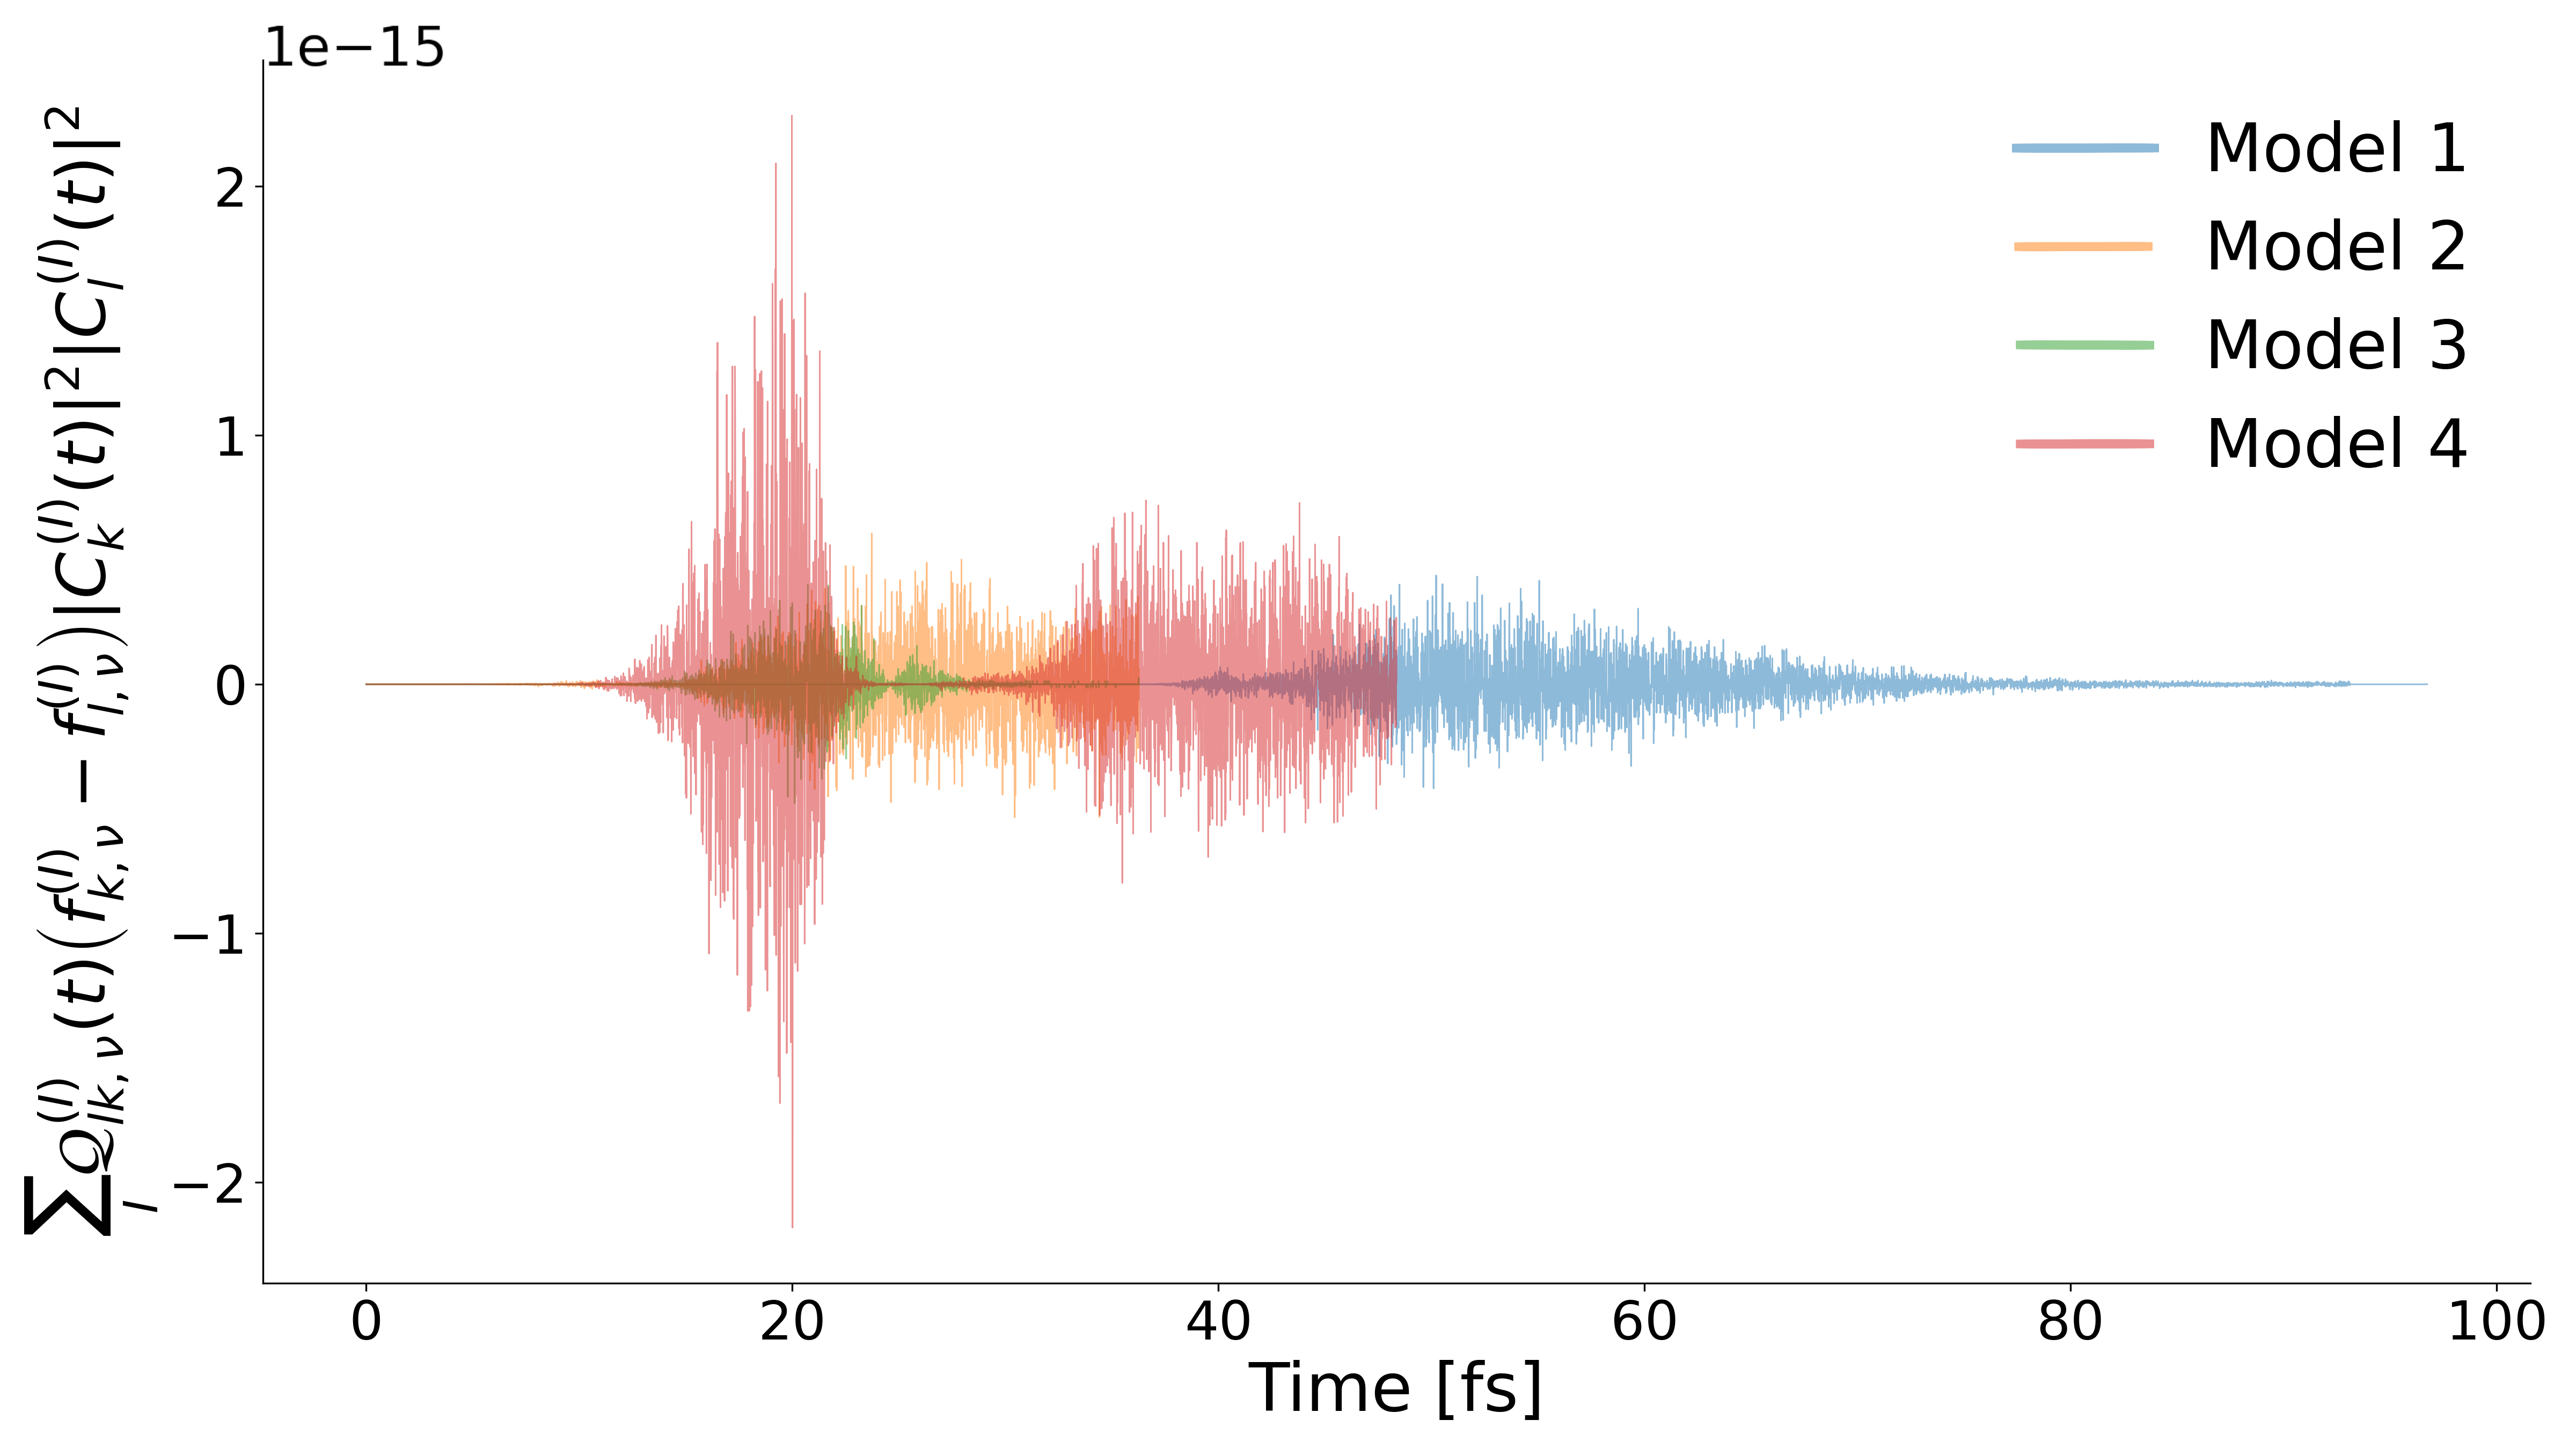
\includegraphics[width=\textwidth]{./img/CTMQC/TullyModels/CTMQC_S27.png}
	\caption{\label{fig:S27}The conserved quantity given in equation \eqref{eq:S27}. Each color represents data outputted by a simulation using a different model (specified in the legend). Each time-series is plotted with a translucent color meaning each model's data can be seen at once.}
\end{figure}

In the SI of Min, 17 \cite{min_ab_2017} a conservation equation (S27) is given. This is repeated below in equation \eqref{eq:S27}
\begin{equation}
	\sum_{I} \mathcal{Q}_{lk, \nu}^{(I)}(t) \left( f_{k, \nu}^{(I)} - f_{l, \nu}^{(I)} \right) |C_{k}^{(I)} (t)|^2 |C_{l}^{(I)} (t)|^2 = 0  \qquad \forall l, k, \nu
	\label{eq:S27}
\end{equation}

An example time-series of this quantity is given in figure \ref{fig:S27} for each Tully model. The data used to calculate come from simulations of each of the Tully models using the parameters given in appendix \ref{app:tully_params}. No smoothing was used for the $\mathbf{R}_{lk, \nu}^{(I)}$ term. It can be seen in this figure that the conservation quantity hovers around 0 for each model with a maximum deviation of 10$^{-15}$ m$_{e}$Ha.

\subsubsection{$\sum_{l} \mathbb{X}_{qm, ll} |C_{l}^{(I)}|^2$}
\label{sect:sumXqmll}
As the equations are currently formulated another numerical test validating the quantum momentum part of the propagation equations for the coefficients can be used. The CTMQC equation for the propagation of the adiabatic expansion coefficients is given in equation \eqref{eq:elec_adiab}. The quantum momentum part of this equation is given below in equation \eqref{eq:qmCTMQCAdiab}. 
\begin{equation}
  \mathbb{X}_{qm, ll}^{(I)} = \sum_{\nu=1}^{N_n}\sum_{k} \frac{\mathcal{Q}_{lk, \nu}^{(I)}}{\hbar     M_\nu} \cdot \left[ \mathbf{f}_{k,\nu}^{(I)} - \mathbf{f}_{l,\nu}^{(I)}   \right] |C_{k}^{(I)}|^2
  \label{eq:qmCTMQCAdiab}
\end{equation}
Where $\mathbb{X}_{qm, ll}^{(I)}$ is the diagonal matrix that, when multiplied with the adiabatic expansion coefficients, gives the quantum momentum contribution to the propagation of the expansion coefficients.I
\\\\
We can test the construction of this matrix within the code by multiplying by the adiabatic populations and summing as shown in equation \eqref{eq:NumericalTestXqmll}. It can be shown, assuming perfect norm conservation, that this should equal exactly 0 -due to the symmetry of the $|C_{l}^{(I)}|^2|C_{k}^{(I)}|^2$ and the quantum momentum matrix. This is checked for every timestep during propagation.

\begin{equation}
  \sum_{l} \mathbb{X}_{qm, ll}^{(I)} |C_{l}^{(I)}|^2 = 0
  \label{eq:NumericalTestXqmll}
\end{equation}


\subsection{Energy Conservation}
\subsubsection{Ehrenfest}
Energy conservation is a very important property in most molecular dynamics simulations. In Ehrenfest of mean-field molecular dynamics nuclei are propagated on a population-weighted mean potential energy surface, e.g. $\sum_{k}|C_{l}^{(I)}(t)|^2 = E_{eff}(t)$ \cite{EhrenEnerCons}. Kinetic energy of the classical nuclei is given by the standard formula, e.g. $\frac{1}{2} m v^2$. We can therefore write down the conserved quantity as defined below in equation \eqref{eq:EhrenfestEnergyConservation}:
\begin{equation}
  \frac{d E}{dt} = \frac{d}{dt} \left[ \frac{1}{2} m v^2 + \sum_{k}|C_{l}^{(I)}(t)|^2 \right] = 0
  \label{eq:EhrenfestEnergyConservation}
\end{equation}
As in the norm conservation checks in section \ref{sect:normCons},  parameters from the high momentum cases were taken as initial conditions for simulations with various nuclear timesteps, this time holding the electronic timestep constant. The high momenta cases were chosen to show the worst case energy conservations, within this very simple system. A linear line of best fit was then fitted to the data and the drift in the total energy (given in \eqref{eq:EhrenfestEnergyConservation}) was calculated from its gradient. The results of these simulations are given in figure \ref{fig:EhrenEnerCons}.
\begin{figure}[h]
  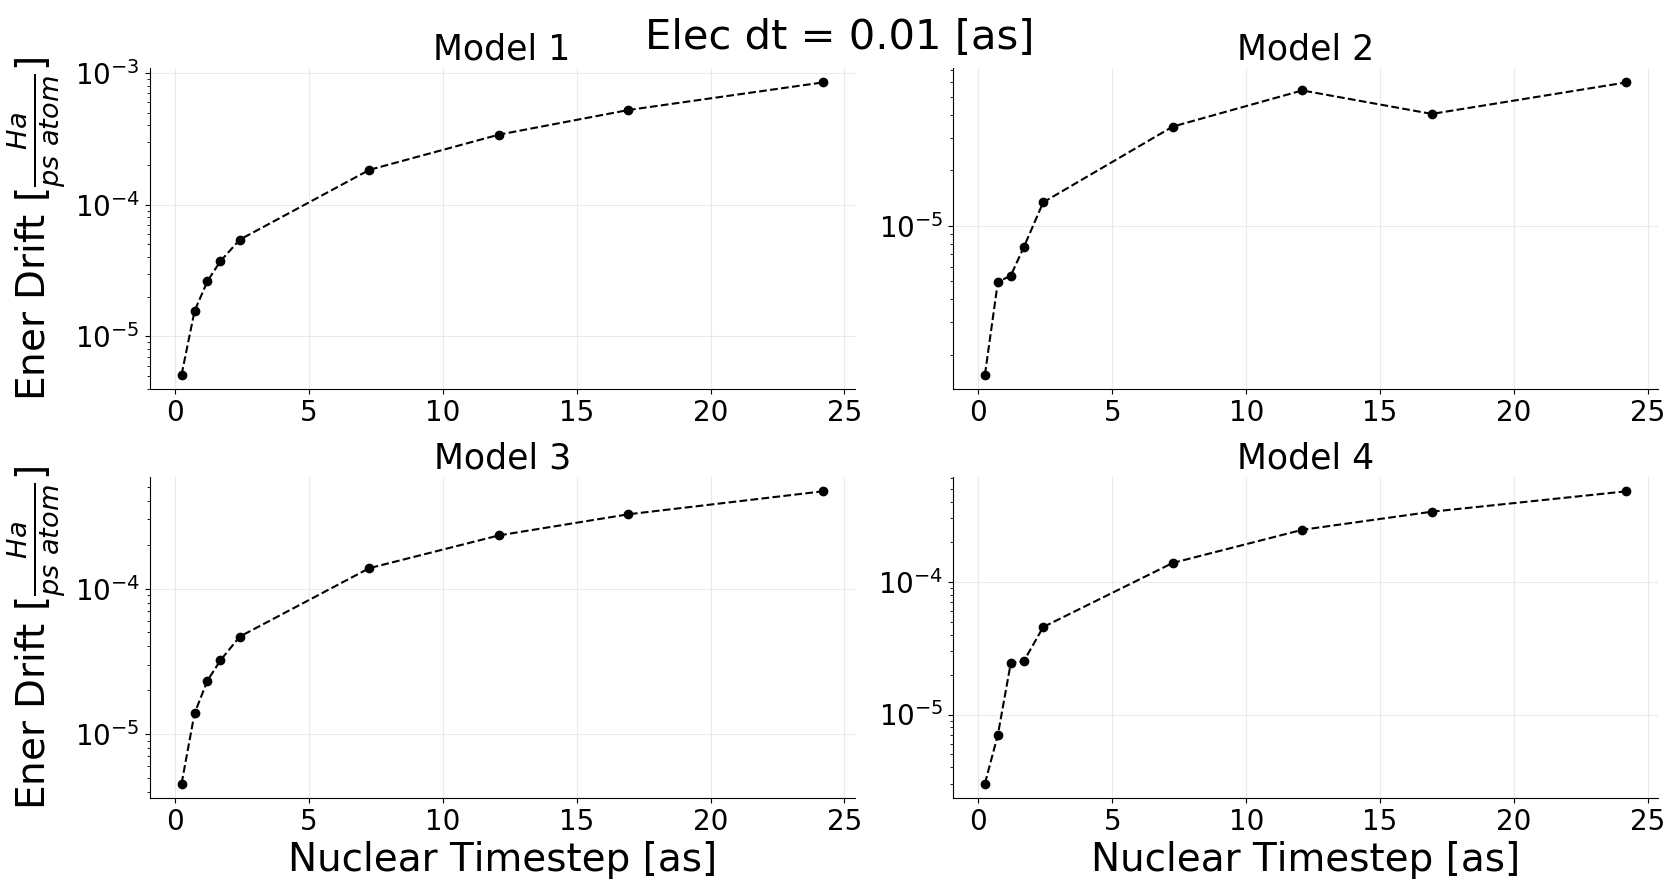
\includegraphics[width=\textwidth]{./img/CTMQC/TullyModels/Ehren_EnerCons.png}
  \caption{\label{fig:EhrenEnerCons}Energy conservation values for various nuclear timesteps for the high momentum case of each Tully model.}
\end{figure}
In figure \ref{fig:EhrenEnerCons}, we see the expected results that as the nuclear timestep is decrease the drift in the total energy also decreases. This trend validates the implementation and shows that in the limit of infinitely small timestep (and infinite computer precision) perfect energy conservation would be achieved. However, fairly small nuclear timesteps are required to achieve reasonable energy conservations. This is because the system contains only 1 atom with a mass comparable to that of Hydrogen. If one needed an improved energy conservation a higher order integrator than the velocity verlet used here may also improve results slightly.
\subsubsection{CTMQC}
In CTMQC the energy conservation is 





\section{Calculation of $\mathcal{Q}_{lk, \nu}^{(I)}$}
\label{sect:SigmaSect}
In order to calculate the quantum momentum the nuclear density must be constructed from the nuclei's positions. However, the nuclei are treated classically, i.e. as point particles. To approximate the nuclear density from atomic positions a normal distribution is placed with the mean at position of each particle with a width of $\sigma$. This introduces a new parameter which must be tuned in order to reproduce sensible results. If the width is too small the resulting nuclear density is too noisy and the quantum momentum values unreliable. If the width is too large the nuclear density is very smooth with little variation and the quantum momentum values become very small. Seeing as the quantum momentum is one of the most important factors affecting coherence between electronic states the careful selection of the $\sigma$ parameter is important. This issue is not very well addressed in the literature. In this section I will show results of calculation carried out with various values of $\sigma$ 
 as well as a method for a dynamic calculation of $\sigma(t)$ on the fly.
 \subsection{Constant Values of $\sigma$}



